\chapter{Menú inicial}
\label{chap:menu}

Antes de empezar a desarrollar la aplicacion se establecieron un icono y una paleta de colores que se utilizaron en toda la aplicacion. 

El icono es el que aparece en la pantalla de inicio y en la barra superior de la aplicacion. 

La paleta de colores se utilizo para establecer los colores de fondo, texto y botones y esta en el archivo \texttt{res/values/colors.xml}.

\begin{figure}[H]
  \centering
  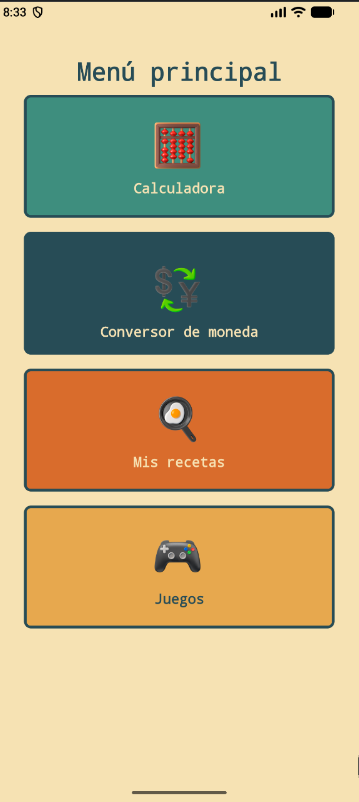
\includegraphics[width=0.4\textwidth]{menu}
\end{figure}